% !Mode:: "TeX:UTF-8:Main"
\documentclass[aspectratio=169]{beamer}

\usepackage{tikz}
\usetikzlibrary{ducks}

\setbeamertemplate{navigation symbols}{}
\setbeamertemplate{background canvas}{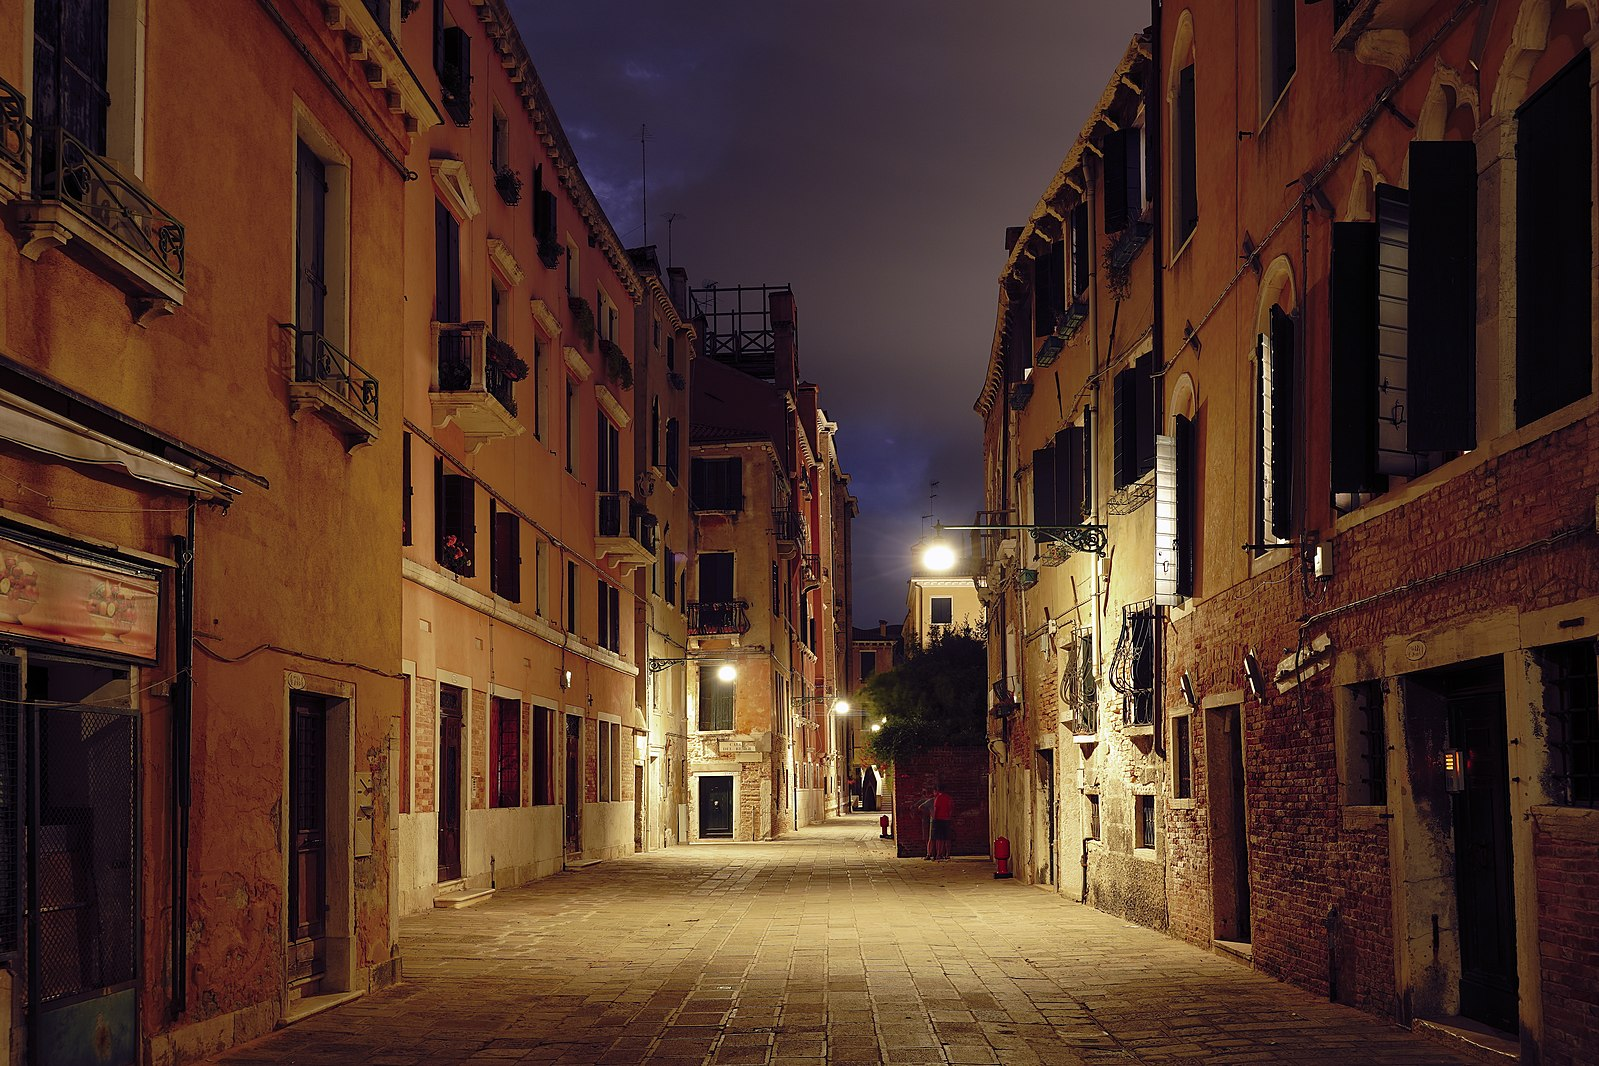
\includegraphics[trim=0cm 0cm 0cm 6cm,width=\paperwidth]{emptyroad}}

% trick taken from https://topanswers.xyz/tex?q=1989
\tikzset{
    use page relative coordinates/.style={
        shift={(current page.south west)},
        x={(current page.south east)},
        y={(current page.north west)}
    },
}

\begin{document}
	
% music 1:20-1:34 -> needs 14*25=350 frames
\begin{frame}
  \begin{tikzpicture}[]
   \path[use as bounding box](0,0)rectangle (\textwidth,\textheight-14.7pt);
    % credit for background image
    \node[white,text width=.7\paperwidth,font=\tiny,align=center] at ([yshift=88mm]current page.south) {Image source: \url{https://commons.wikimedia.org/wiki/File:Venezia_Venice_summer_2019_147.jpg}};  
    
     
    \path (\fpeval{130-\value{page}/350*170}mm,-0.1) pic[duck/grumpy]
      {duck};
  
  \end{tikzpicture}
  \pause[350]
\end{frame}	
	\setbeamertemplate{background canvas}{%
      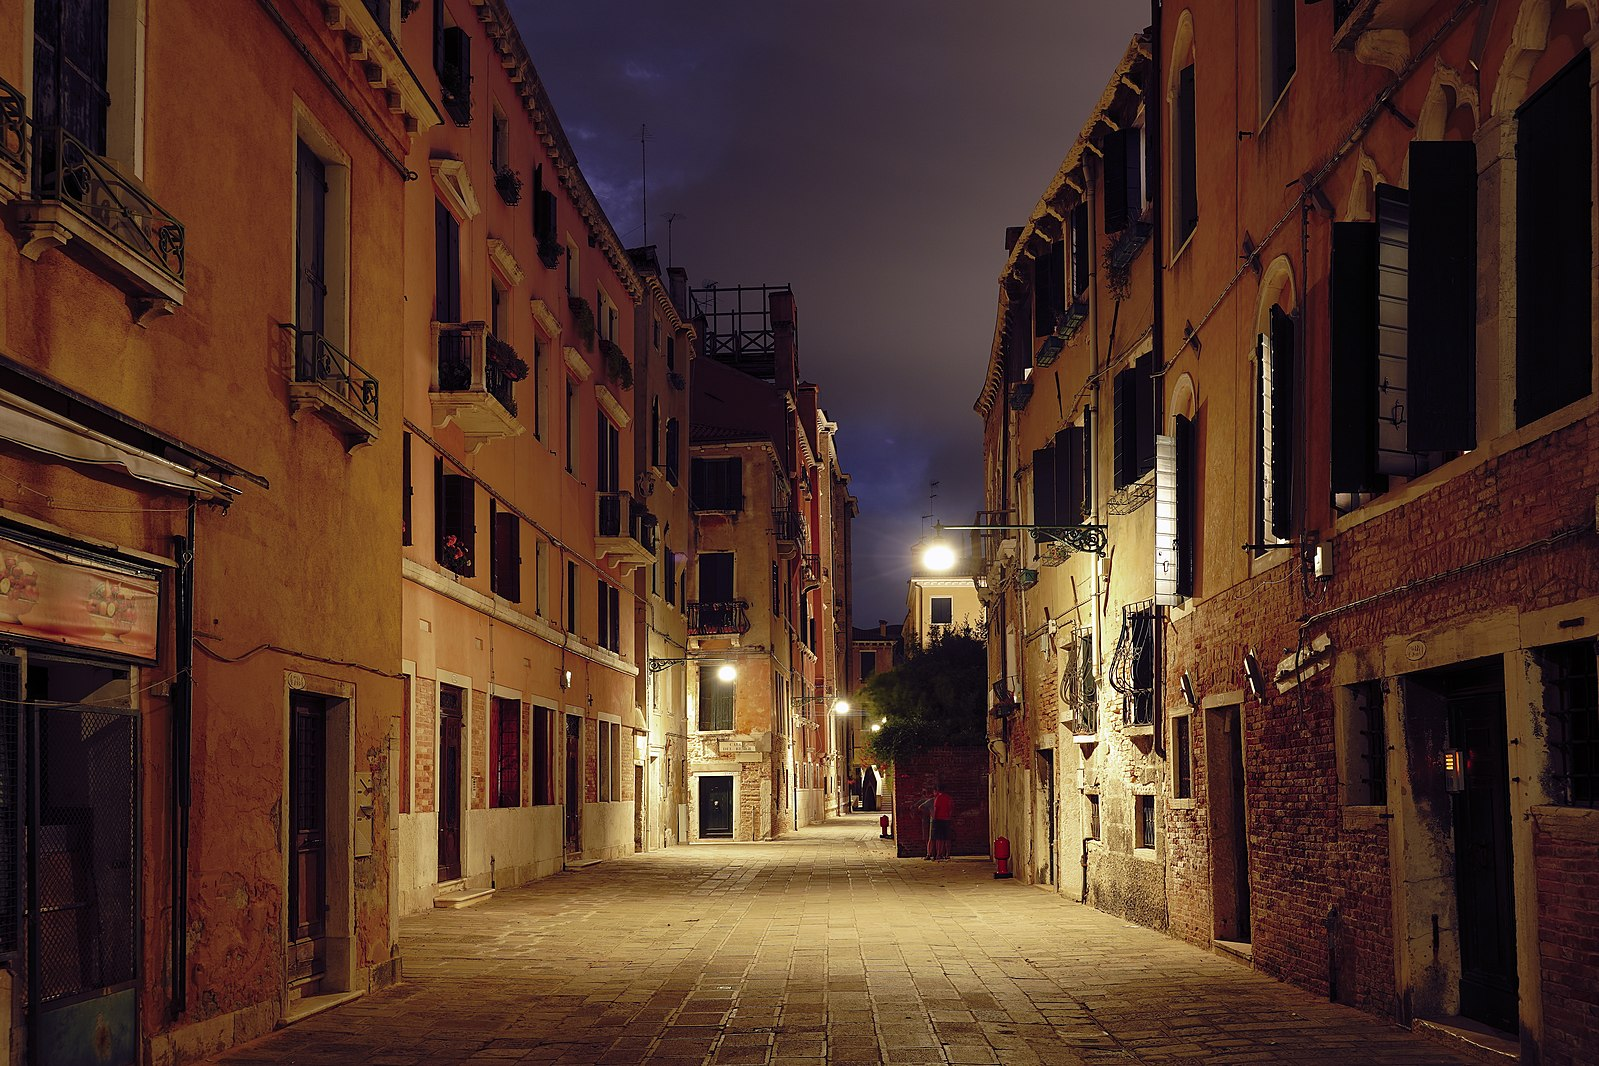
\includegraphics[trim=0cm 0cm 0cm 6cm,width=\paperwidth]{emptyroad}%
      \llap{\makebox[\paperwidth]{%
      \scalebox{0.7}[0.4]{%
      \begin{tikzpicture}[overlay] 
            \path[clip] (-0.24\paperwidth,0)--++ (0.48\paperwidth,0)--++(-1,4cm)--++(-2cm,4.5cm)
       --++(-3cm,-4cm)--cycle ;
    
      \node[anchor=south,inner sep=0pt,opacity=\fpeval{(\value{page}-200)/40}]{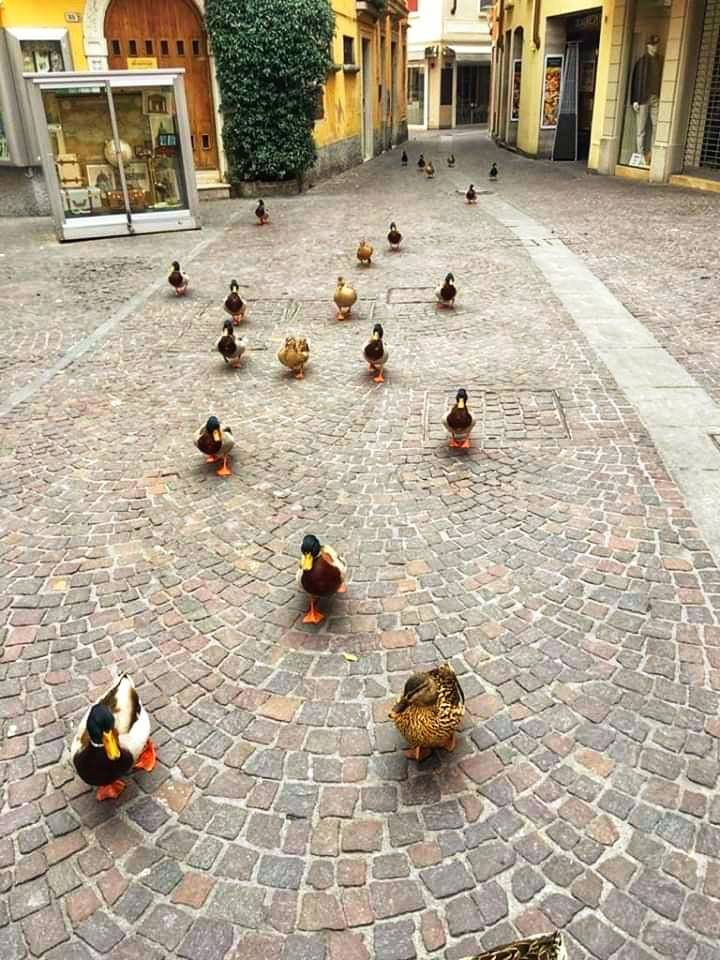
\includegraphics[height=\paperheight,trim=0cm 4cm 0cm 0cm]{ducksmarch}};
      \end{tikzpicture}} }}} 

% music 1:34-1:53 -> needs 19*25=475 frames
\begin{frame}[label=quack]
  \begin{tikzpicture}
  \path[use as bounding box](0,0)rectangle (\textwidth,\textheight-14.7pt);
\node[white,text width=.7\paperwidth,font=\tiny,align=center] at ([yshift=88mm]current page.south) {Image source: \url{https://commons.wikimedia.org/wiki/File:Venezia_Venice_summer_2019_147.jpg}};  
    

    % credit for background image
    % \node[white,text width=.7\paperwidth,font=\tiny,align=center] at ([yshift=0.35cm]current page.south) {Image source: ??};  
  \path (\fpeval{-20+(\value{page}-200)/350*80}mm,-0.1) pic[xscale=-1]
      {duck};
  \end{tikzpicture}
  \pause[475]
\end{frame}	

\end{document}
